\documentclass{standalone}
\usepackage{tikz}
\usetikzlibrary{patterns, positioning}
\usepackage[sfdefault]{ClearSans} %% option 'sfdefault' activates Clear Sans as the default text font
\usepackage[T1]{fontenc}

\begin{document}
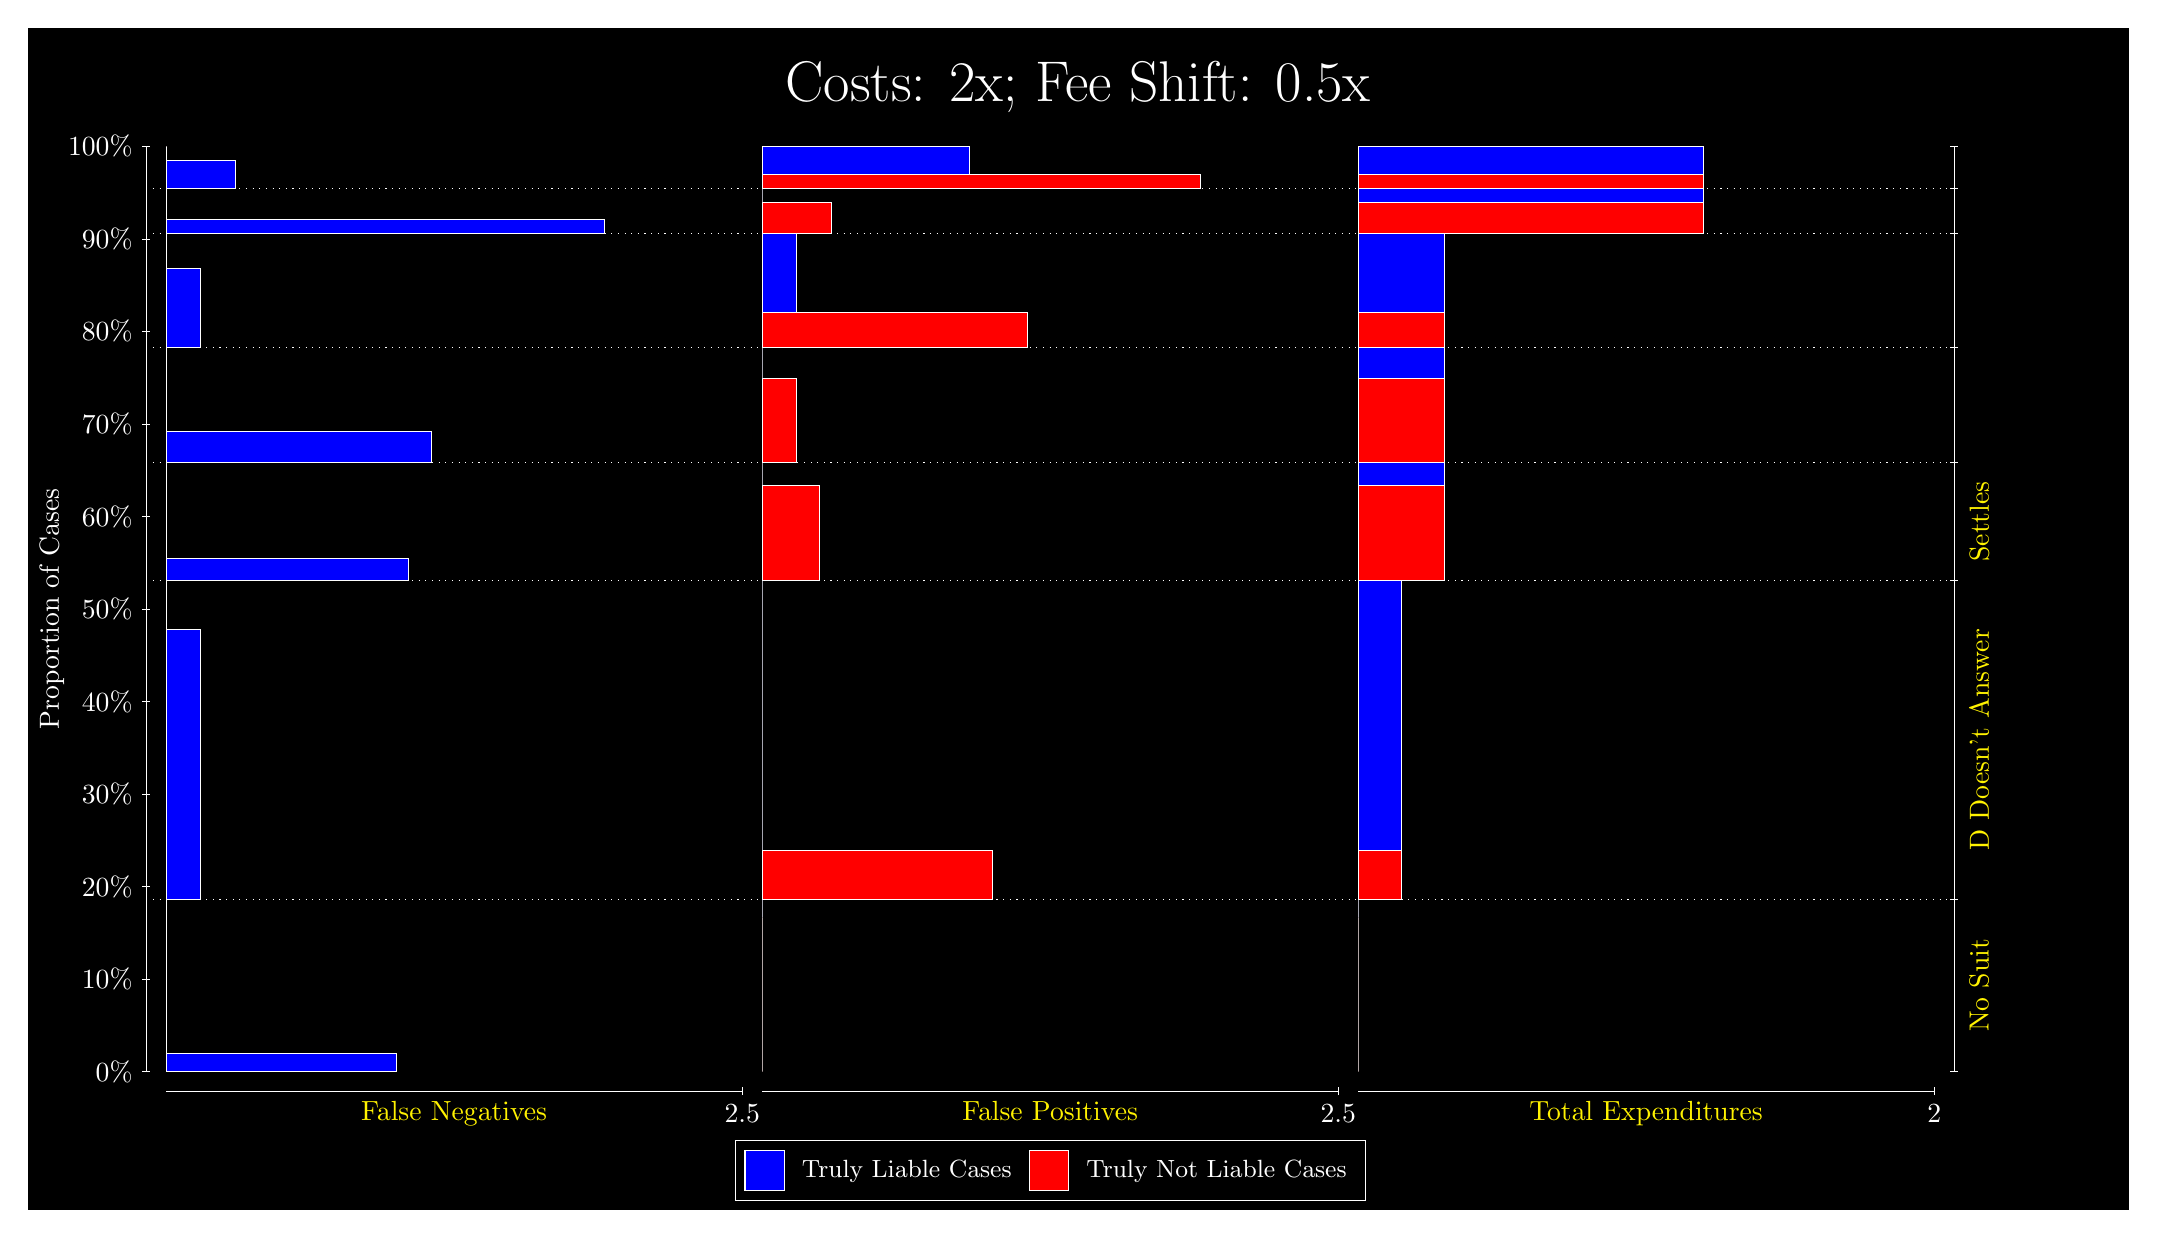
\begin{tikzpicture}
\draw[fill=black] (0,0) rectangle (26.667,15);
\draw[text=white] (0,13.5) rectangle (26.667,15) node[midway] {\huge Costs: 2x; Fee Shift: 0.5x};
\draw[white, very thin] (1.5,1.75) -- (1.5,13.5);
\node[rotate=90, text=white, anchor=center] at (0.3, 7.625) {Proportion of Cases};
\draw[white, very thin] (1.45,1.75) -- (1.55,1.75);
\node[text=white, anchor=east] at (1.45, 1.75) {0\%};
\draw[white, very thin] (1.45,2.925) -- (1.55,2.925);
\node[text=white, anchor=east] at (1.45, 2.925) {10\%};
\draw[white, very thin] (1.45,4.1) -- (1.55,4.1);
\node[text=white, anchor=east] at (1.45, 4.1) {20\%};
\draw[white, very thin] (1.45,5.275) -- (1.55,5.275);
\node[text=white, anchor=east] at (1.45, 5.275) {30\%};
\draw[white, very thin] (1.45,6.45) -- (1.55,6.45);
\node[text=white, anchor=east] at (1.45, 6.45) {40\%};
\draw[white, very thin] (1.45,7.625) -- (1.55,7.625);
\node[text=white, anchor=east] at (1.45, 7.625) {50\%};
\draw[white, very thin] (1.45,8.8) -- (1.55,8.8);
\node[text=white, anchor=east] at (1.45, 8.8) {60\%};
\draw[white, very thin] (1.45,9.975) -- (1.55,9.975);
\node[text=white, anchor=east] at (1.45, 9.975) {70\%};
\draw[white, very thin] (1.45,11.15) -- (1.55,11.15);
\node[text=white, anchor=east] at (1.45, 11.15) {80\%};
\draw[white, very thin] (1.45,12.325) -- (1.55,12.325);
\node[text=white, anchor=east] at (1.45, 12.325) {90\%};
\draw[white, very thin] (1.45,13.5) -- (1.55,13.5);
\node[text=white, anchor=east] at (1.45, 13.5) {100\%};

\draw[white, very thin] (24.457,1.75) -- (24.457,13.5);
\draw[white, very thin] (24.407,1.75) -- (24.507,1.75);
\node[anchor=west] at (24.407, 1.75) {};
\draw[white, very thin] (24.407,3.9363) -- (24.507,3.9363);
\node[anchor=west] at (24.407, 3.9363) {};
\draw[white, very thin] (24.407,7.9871) -- (24.507,7.9871);
\node[anchor=west] at (24.407, 7.9871) {};
\draw[white, very thin] (24.407,9.4835) -- (24.507,9.4835);
\node[anchor=west] at (24.407, 9.4835) {};
\draw[white, very thin] (24.407,10.949) -- (24.507,10.949);
\node[anchor=west] at (24.407, 10.949) {};
\draw[white, very thin] (24.407,12.392) -- (24.507,12.392);
\node[anchor=west] at (24.407, 12.392) {};
\draw[white, very thin] (24.407,12.967) -- (24.507,12.967);
\node[anchor=west] at (24.407, 12.967) {};
\draw[white, very thin] (24.407,13.5) -- (24.507,13.5);
\node[anchor=west] at (24.407, 13.5) {};

\draw[white, very thin, fill=blue] (1.75,1.75) rectangle (4.6775,1.98);
\draw[white, very thin, fill=red] (1.75,1.98) rectangle (1.75,3.9363);
\draw[white, very thin, fill=blue] (1.75,3.9363) rectangle (2.1891,7.3618);
\draw[white, very thin, fill=red] (1.75,7.3618) rectangle (1.75,7.9871);
\draw[white, very thin, fill=blue] (1.75,7.9871) rectangle (4.8239,8.2698);
\draw[white, very thin, fill=red] (1.75,8.2698) rectangle (1.75,9.4835);
\draw[white, very thin, fill=blue] (1.75,9.4835) rectangle (5.1167,9.8839);
\draw[white, very thin, fill=red] (1.75,9.8839) rectangle (1.75,10.949);
\draw[white, very thin, fill=blue] (1.75,10.949) rectangle (2.1891,11.952);
\draw[white, very thin, fill=red] (1.75,11.952) rectangle (1.75,12.392);
\draw[white, very thin, fill=blue] (1.75,12.392) rectangle (7.3123,12.569);
\draw[white, very thin, fill=red] (1.75,12.569) rectangle (1.75,12.967);
\draw[white, very thin, fill=blue] (1.75,12.967) rectangle (2.6283,13.323);
\draw[white, very thin, fill=red] (1.75,13.323) rectangle (1.75,13.5);
\draw[white, very thin, fill=red] (9.3189,1.75) rectangle (9.3189,3.7063);
\draw[white, very thin, fill=blue] (9.3189,3.7063) rectangle (9.3189,3.9363);
\draw[white, very thin, fill=red] (9.3189,3.9363) rectangle (12.246,4.5616);
\draw[white, very thin, fill=blue] (9.3189,4.5616) rectangle (9.3189,7.9871);
\draw[white, very thin, fill=red] (9.3189,7.9871) rectangle (10.051,9.2008);
\draw[white, very thin, fill=blue] (9.3189,9.2008) rectangle (9.3189,9.4835);
\draw[white, very thin, fill=red] (9.3189,9.4835) rectangle (9.758,10.549);
\draw[white, very thin, fill=blue] (9.3189,10.549) rectangle (9.3189,10.949);
\draw[white, very thin, fill=red] (9.3189,10.949) rectangle (12.686,11.389);
\draw[white, very thin, fill=blue] (9.3189,11.389) rectangle (9.758,12.392);
\draw[white, very thin, fill=red] (9.3189,12.392) rectangle (10.197,12.79);
\draw[white, very thin, fill=blue] (9.3189,12.79) rectangle (9.3189,12.967);
\draw[white, very thin, fill=red] (9.3189,12.967) rectangle (14.881,13.144);
\draw[white, very thin, fill=blue] (9.3189,13.144) rectangle (11.954,13.5);
\draw[white, very thin, fill=red] (16.888,1.75) rectangle (16.888,3.7063);
\draw[white, very thin, fill=blue] (16.888,3.7063) rectangle (16.888,3.9363);
\draw[white, very thin, fill=red] (16.888,3.9363) rectangle (17.437,4.5616);
\draw[white, very thin, fill=blue] (16.888,4.5616) rectangle (17.437,7.9871);
\draw[white, very thin, fill=red] (16.888,7.9871) rectangle (17.986,9.2008);
\draw[white, very thin, fill=blue] (16.888,9.2008) rectangle (17.986,9.4835);
\draw[white, very thin, fill=red] (16.888,9.4835) rectangle (17.986,10.549);
\draw[white, very thin, fill=blue] (16.888,10.549) rectangle (17.986,10.949);
\draw[white, very thin, fill=red] (16.888,10.949) rectangle (17.986,11.389);
\draw[white, very thin, fill=blue] (16.888,11.389) rectangle (17.986,12.392);
\draw[white, very thin, fill=red] (16.888,12.392) rectangle (21.279,12.79);
\draw[white, very thin, fill=blue] (16.888,12.79) rectangle (21.279,12.967);
\draw[white, very thin, fill=red] (16.888,12.967) rectangle (21.279,13.144);
\draw[white, very thin, fill=blue] (16.888,13.144) rectangle (21.279,13.5);
\draw[white, dotted] (1.5,3.9363) -- (24.457,3.9363);
\draw[white, dotted] (1.5,7.9871) -- (24.457,7.9871);
\draw[white, dotted] (1.5,9.4835) -- (24.457,9.4835);
\draw[white, dotted] (1.5,10.949) -- (24.457,10.949);
\draw[white, dotted] (1.5,12.392) -- (24.457,12.392);
\draw[white, dotted] (1.5,12.967) -- (24.457,12.967);
\draw[white, very thin] (1.75,1.5) -- (9.0689,1.5);
\node[text=yellow, anchor=north] at (5.4094, 1.5) {False Negatives};
\draw[white, very thin] (9.0689,1.45) -- (9.0689,1.55);
\node[text=white, anchor=north] at (9.0689, 1.45) {2.5};

\draw[white, very thin] (9.3189,1.5) -- (16.638,1.5);
\node[text=yellow, anchor=north] at (12.978, 1.5) {False Positives};
\draw[white, very thin] (16.638,1.45) -- (16.638,1.55);
\node[text=white, anchor=north] at (16.638, 1.45) {2.5};

\draw[white, very thin] (16.888,1.5) -- (24.207,1.5);
\node[text=yellow, anchor=north] at (20.547, 1.5) {Total Expenditures};
\draw[white, very thin] (24.207,1.45) -- (24.207,1.55);
\node[text=white, anchor=north] at (24.207, 1.45) {2};

\node[text=yellow, centered, rotate=90] at (24.777, 2.8432) {No Suit};
\node[text=yellow, centered, rotate=90] at (24.777, 5.9617) {D Doesn't Answer};
\node[text=yellow, centered, rotate=90] at (24.777, 8.7353) {Settles};





\draw (12.978300999999998,1.5) node[draw=none] (baseCoordinate) {};
\begin{scope}[align=center]
        \matrix[scale=0.5, draw=white, below=0.5cm of baseCoordinate, nodes={draw}, column sep=0.1cm]{
            \node[rectangle, draw, minimum width=0.5cm, minimum height=0.5cm, fill=blue] {}; &
            \node[draw=none, font=\small, text=white] (B) {Truly Liable Cases}; &
            \node[rectangle, draw, minimum width=0.5cm, minimum height=0.5cm, fill=red] {}; &
            \node[draw=none, font=\small, text=white] (B) {Truly Not Liable Cases}; \\
            };
\end{scope}

\end{tikzpicture}
\end{document}